%--------------------------------TOP LEVEL SHIT-------------------------------------------------------------------------------
\documentclass[11pt, oneside]{article}   
\usepackage{geometry}                		
\geometry{letterpaper}                   		
\usepackage{graphicx}    
\usepackage{amssymb}
\usepackage{enumerate}
%--------------------------------------------------------------------------------------------------------------------------------------
\title{Sfwr Eng 2XB3 - Final Project}    
\author{ 
	Group 33  - The Scrabbler \\ \\         
	Greg Barkans \\
	Colin Gillespie \\
	Curtis Milos \\
	 \vspace{1cm} \\
	Prof: Dr. Samavi \\
	Lab: L01 \\
	Due: Friday April 10, 2015 \\
	\vspace{1cm} \\
}
\date{}		 			
%--------------------------------------------------------------------------------------------------------------------------------------
\begin{document}    
\maketitle                  

\textbf{NOTE:} An official Testing Report was NOT mentioned in the final project requirements, but since we had to perform testing anyways our group included this as proof.  We also did our entire implementation from scratch (including our own data structures etc) and didn't rely on libraries and thus testing our implementation is very critical. 
\newpage     
\tableofcontents   
\newpage             
\listoffigures         
\newpage
\listoftables
\newpage

%------------------------------------------------------SECTION 1-----------------------------------------------------------------

\section*{Preface}
This document is organized with each chapter dedicated to a different testing procedure type (from low-level unit testing to higher level system testing).  Within each chapter,  there is a section representing a conceptual model.  From there, there are subsections for each class module and sub subsections for each unit/method within those classes.  


%----------------------------------------------------------------------------------------------------------------------------------------
%------------------------------------------------------CHAPTER 1-----------------------------------------------------------------
%----------------------------------------------------------------------------------------------------------------------------------------

\section{Unit Testing}
%-- Intro paragraph
The manner in which each of these tests were done was systemically consist.  Specifically, each unit was tested on its own with necessary stubs and drivers.  This sort of testing is considered to be whitebox and will verify the method on its own, but will not imply integration/system testing (to be done in other ways).  This manner of testing will verify the \textsc{functional correctness} of the requirements for the particular method, and only that method.

%-----------------------Chapter 1, section 1: Model----%
\subsection{Model}
The model contains methods that generate regular expression based off of how the user initializes the board with letters and highlighting.  These methods use the BST and Trie table data structures.  As such, these methods are very complex.  In order to verify that the methods are working separately from the data structures (and especially since data structures are often changeable qualities of a software product), these methods were tested with drivers and stubs.  A Testing.html file was setup and any values that were to reside in the data structures or be given to these methods by external methods were hard coded in.  

%-----hl Indicies
\begin{table}[hl]
\caption{private method this.hlIndicies}
\begin{center}
\begin{tabular}{|p{0.25\textwidth}|p{0.3\textwidth}|p{0.3\textwidth}|p{0.05\textwidth}|}

\hline
\textbf{TEST CASE} & \textbf{EXPECTED RESULT} & \textbf{ACTUAL RESULT} & P/F \\
\hline
d: ``horizontal" x:3, y:4 with 3 highlighted cells and no letters & [0, 1, 2] & [0, 1, 2] & P \\
\hline
d: ``vertical" x:1, y:1 with 4 highlighted cells and a letter in the second one & [0,2,3] & [0,2,3] & P \\
\hline
d: ``horizontal" x:0, y:0 with 7 highlighted cell and a letter in the first and last cell & [1, 2, 3, 4, 5] & [1, 2 , 3 ,4 ,5] & P \\
\hline
\end{tabular}
\end{center}
\label{default}
\end{table}%

%-----match Tiles
\begin{table}[hl]
\caption{public method this.matchTiles}
\begin{center}
\begin{tabular}{|p{0.25\textwidth}|p{0.3\textwidth}|p{0.3\textwidth}|p{0.05\textwidth}|}

\hline
\textbf{TEST CASE} & \textbf{EXPECTED RESULT} & \textbf{ACTUAL RESULT} & P/F \\
\hline
words in heap: side, dies, ides, peep. Horizontal highlight from [0][0] to [0][3]. Tiles: s,i,d,e
& [side, ides, dies] & [side, ides, dies] & P \\
\hline
words in heap: side, dies, ides, peep. Horizontal highlight from [0][0] to [0][3]. Tiles: none & [ ] & [ ] & P \\
\hline
words in heap: side, dies, ides, peep. Horizontal highlight from [0][0] to [0][3]. Tiles: i,d,e,wildcard & [side, ides, dies] & [sides, ides, dies] & P \\
\hline


\hline
\end{tabular}
\end{center}
\label{default}
\end{table}%

%----create Regex
\begin{table}[hl]
\caption{public method this.matchTiles}
\begin{center}
\begin{tabular}{|p{0.25\textwidth}|p{0.3\textwidth}|p{0.3\textwidth}|p{0.05\textwidth}|}

\hline
\textbf{TEST CASE} & \textbf{EXPECTED RESULT} & \textbf{ACTUAL RESULT} & P/F \\
\hline
cells [0][0] to [0][3] highlighted, no letters & /\textbackslash w \textbackslash w \textbackslash w \textbackslash w/ & /\textbackslash w \textbackslash w \textbackslash w \textbackslash w/ & P \\
\hline
cells [1][2] to [4][2] highlighted, an a in cell [1][2] & / a \textbackslash w \textbackslash w \textbackslash w / & / a \textbackslash w \textbackslash w \textbackslash w / & P \\
\hline
cells[2][2] to [5][2] highlight, an a in cell [2][2], a b in cell [3][1] & / a [aeioy] \textbackslash w \textbackslash w / & / a [aeioy] \textbackslash w \textbackslash w / & P \\
\hline
\end{tabular}
\end{center}
\label{default}
\end{table}%

\begin{figure}[hl]
\caption{console log of regex generater testing an edge case}
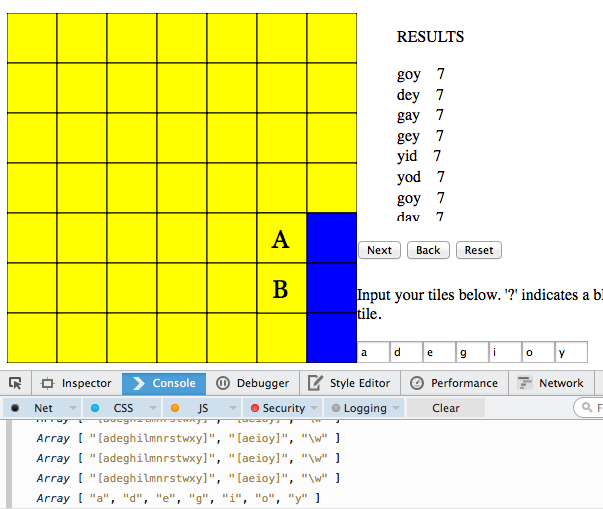
\includegraphics[width=0.95\textwidth]{regex.png}
\end{figure}

%-----------------------Chapter 1, section 2: View----%
\section{System \& Integration Testing (BlackBox)}
Both the view and the controller are a lot harder to test in a white-box driver/stub system.  As such, they were black-box tested after integration with the model.  The view itself doesn't contain many methods and mostly deals with drawing the canvas.  We haven't implemented many css scalable features, so there isn't too much to test as of yet.  The controller is tested via canonical sequences of the HTML buttons (back, next, reset).  

\subsection{View}
The view contains methods that update:
\begin{enumerate}[1)]
	\item The HTML canvas (the grid the user sees)
	\item The paragraph telling the user what to do
	\item The result div beside the grid
\end{enumerate}


\begin{figure}[hl]
\caption{The View}
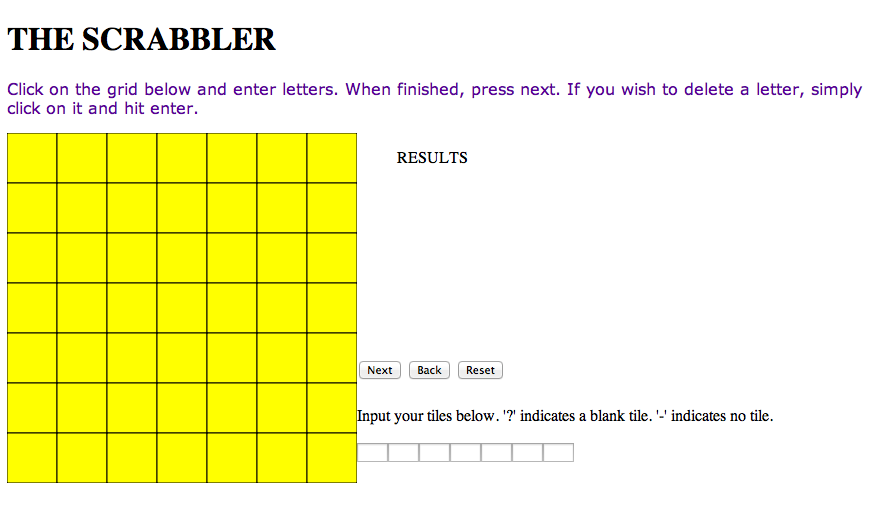
\includegraphics[width=0.95\textwidth]{view.png}
\end{figure}




%-----------------------Chapter 1, section 3: Controller----%
\subsection{Controller}
The controller is responsible for calling the appropriate function based on the buttons the user presses.  These buttons are:
\begin{enumerate}[1)]
	\item back
	\item next
	\item reset
\end{enumerate}

Additionally, it also listens to the form query representing the user's tiles (the input boxes on the bottom right), as well as sends other document information to the View and Model as necessary.  This is to minimize the interaction the Model and View have with the HTML to a uni-directional uses relationship and modularize/separate concerns.  

\begin{figure}[hl]
\caption{Controller: initial and highlight states}
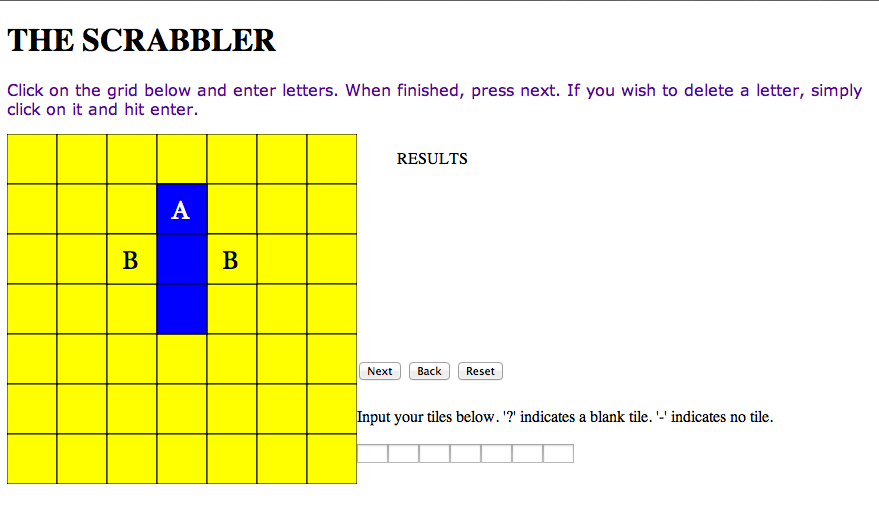
\includegraphics[width=0.95\textwidth]{c1.png}
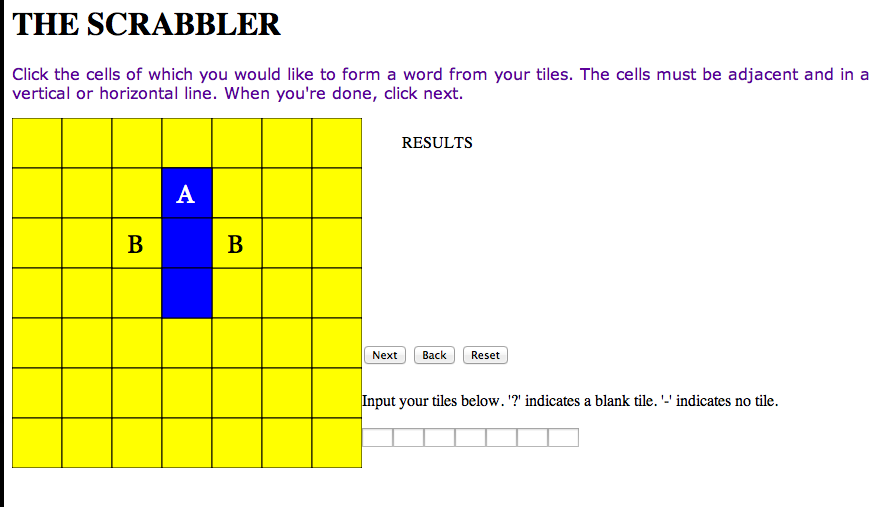
\includegraphics[width=0.95\textwidth]{c2.png}
\end{figure}

\begin{figure}[hl]
\caption{Controller: tile state and error alert}
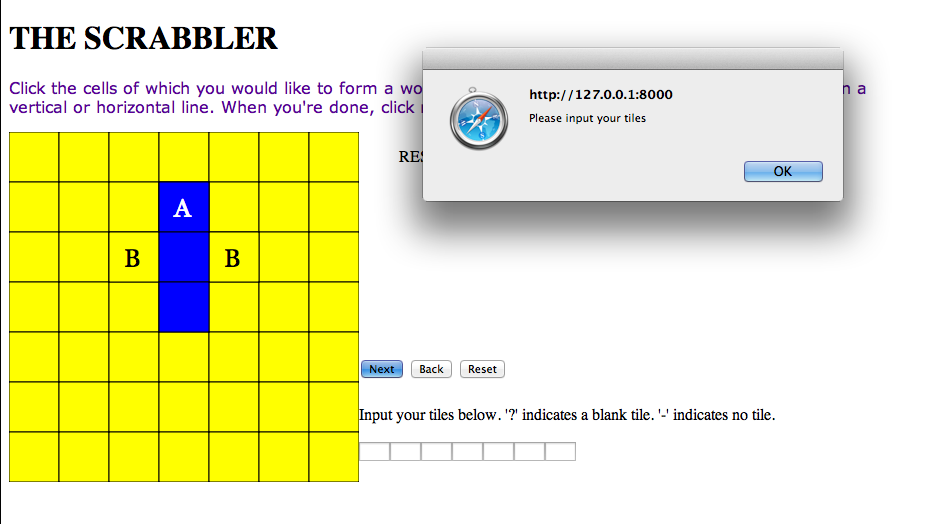
\includegraphics[width=0.95\textwidth]{c3.png}
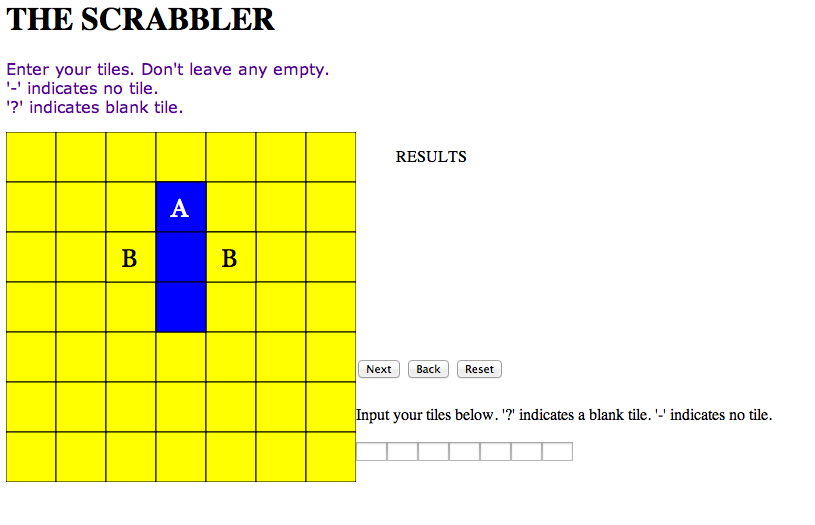
\includegraphics[width=0.95\textwidth]{c4.png}
\end{figure}

\begin{figure}[hl]
\caption{Controller: Result state}
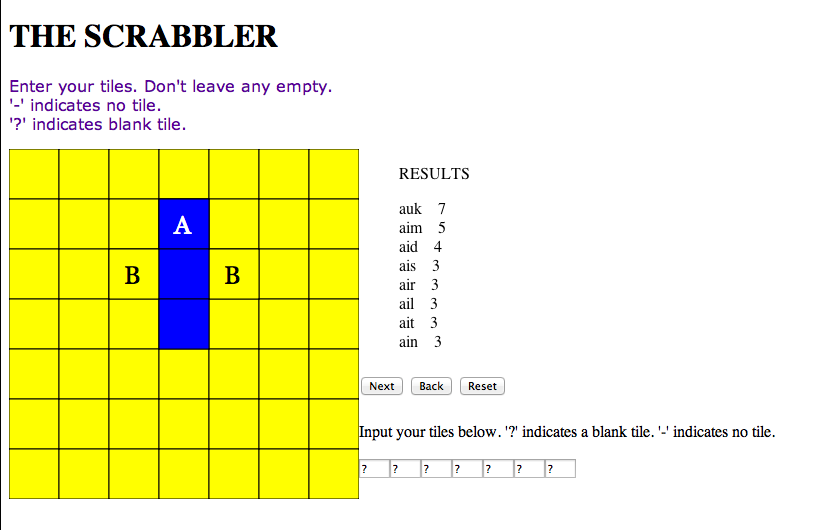
\includegraphics[width=0.95\textwidth]{c5.png}
\end{figure}


%----------------------------------------------------------------------------------------------------------------------------------------
%------------------------------------------------------CHAPTER 1-----------------------------------------------------------------
%----------------------------------------------------------------------------------------------------------------------------------------

\end{document}  